% toc=listof sorgt dafür, dass Abbildungs- und Tabellenverzeichnis
% mit einem Eintrag im Inhaltsverzeichnis aufgeführt werden.
\documentclass[11pt,a4paper,toc=listof]{scrreprt}

\newcommand{\WS}{William Shakespeare}

\newcommand{\Rolle}[1]{\textbf{#1}}

\newcommand{\Ausruf}[1]{\textit{#1}}
\usepackage[utf8]{inputenc}
\usepackage[T1]{fontenc}
\usepackage[ngerman]{babel}

% Anstatt das Deckblatt manuell mit \huge und \tiny zu formatieren, sollten wir
% besser LaTeX diese Aufgabe übernehmen lassen. Wir müssen lediglich die
% Metainformationen mit den entsprechenden Befehlen definieren und später reicht
% eine einzige Zeile, um ein nettes Deckblatt zu erstellen.
\title{Hamlet -- Prinz von Dänemark}
\author{William Shakespeare}
% Der Befehl \today gibt das aktuelle Datum aus und wird bei jedem Kompilieren
% aktualisiert.
\date{\today{}}

\begin{document}

\begin{titlepage}
\maketitle
\end{titlepage}

\tableofcontents
% Hier werden Abbildungs- und Tabellenverzeichnis erzeugt.
\listoffigures
\listoftables

\chapter{Komplexe Inhaltselemente}

\section{Punktliste}

\begin{itemize}
  \item Hamlet
  \item Romeo und Julia
  \item Julius Cäsar
\end{itemize}

\section{Geordnete Liste}

\begin{enumerate}
  \item Hamlet
  \item Romeo und Julia
  \item Julius Cäsar
\end{enumerate}

\section{Definitionsliste}

\begin{description}
  \item [Hamlet] Die Szene ist in Helsingör, nur in der vierten Szene des
  vierten Aktes eine Ebene in Dänemark.
  \item [Romeo und Julia] Die Szene ist im Anfang des fünften Aufzugs in
  Mantua, und sonst immer in Verona.
  \item [Julius Cäsar] Rom, das Lager der Verschwörer nahe Sardis und die Ebenen
  von Philippi.
\end{description}

\section{Geschachtelte Liste}

\begin{enumerate}
\item Hamlet
  \begin{itemize}
  \item König
  \item Ophelia
  \item Hamlet
  \end{itemize}
\item Romeo und Julia
\item Julius Cäsar
\end{enumerate}

\section{Tabellen}

\begin{table}[htb]
  \caption{Die Werke des \WS}
  \label{tab:Werke}
  \begin{tabular}{|l|c|r|}
    \hline
    \textbf{Werk} & \textbf{Autor} & \textbf{Rollen}\\
    \hline
    Hamlet & \WS & Hamlet, Ophelia, König\\
    \hline
    Julius Cäsar & \WS & Julius Cäsar, Brutus\\
    \hline
    Romeo und Julia & \WS & Romeo, Julia\\
    \hline
  \end{tabular}
\end{table}

\newpage

\section{Abbildungen}

\begin{figure}[htb]
\caption{Portrait von \WS}
\label{fig:Portrait}
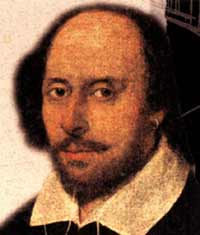
\includegraphics[scale=0.5]{Bilder/Shakespeare.jpg}
\end{figure}

\begin{figure}[htb]
\caption{Logo der ALTE OLDENBURGER (Bitmap, pixelig bei Vergrößerung)}

\includegraphics[scale=0.3]{Bilder/LogoAO.jpg}
\end{figure}
\begin{figure}[htb]
\caption{Logo der ALTE OLDENBURGER (Vektor, ohne Qualitätsverlust skalierbar)}

\includegraphics[scale=0.8]{Bilder/LogoAO.pdf}
\end{figure}

\section{Mathematische Formeln}

Eine Formel mitten im Fließtext ist $y=mx+b$ und hier geht es weiter.

Lange Formeln werden geklammert:
\( \int\limits_a^b {\frac{d}{dx}F(x)dx} = F(b)-F(a) \)

Und viele Formeln mit Nummerierung erzeugt man mit equation:
\begin{equation}
e=mc^2
\end{equation}

\begin{equation}
u(x,t)= 8 \frac{k_{1}^{2}e^{\alpha_{1}} + k_{2}^{2}e^{\alpha_{2}} + (k_{1}-k_{2})^{2}e^{(\alpha_{1}+ \alpha_{2})} \left[2 + \frac{1}{(k_{1} + k_{2})^{2}} ( k_{1}^{2}e^{\alpha_{1}} + k_{2}^{2}e^{\alpha_{2}}) \right]}{\left[1+e^{\alpha_{1}} + e^{\alpha_{2}} + \left(\frac{k_{1} - k_{2}}{k_{1}+k_{2}} \right)^{2} e^{\alpha_{1}+ \alpha_{2}} \right]^{2}}
\end{equation}

\section{URLs}
\url{http://blog.stefan-macke.com}
\chapter{Biographie von \WS}

Ungeachtet der Frage, ob Shakespeare wirklich der Verfasser der ihm
zugeschriebenen Werke war, ist zumindest seine Existenz bezeugt. Leider auch
nicht soviel mehr - was zum einen die altbekannte Frage um die Urheberschaft
seiner Werke aufwirft, zum anderen den Kinoerfolg "`Shakespeare in Love"'
gestattete, sein ganz eigenes Bild des Barden zu entwerfen.

\section[Die Erzeuger]{Die Eltern}
\label{sec:Eltern}

Obwohl Shakespeares Leben besser bezeugt ist als das vieler seiner
Zeitgenossen, lässt sich seine Biographie nur in groben Umrissen rekonstruieren
-- besonders was die Zeit seiner späten Jugend betrifft. \WS
wurde laut Kirchregister am 26. April 1564 in Stratford-on-Avon, Warwickshire,
getauft, sein Geburtstag wird heute der Einfachheit halber auf den 23. April
datiert -- ist Shakespeare doch am gleichen Tage des Jahres 1616 verstorben.

Kommen wir nun zu seinem Vater (siehe Kapitel \ref{sub:Vater} auf Seite
\pageref{sub:Vater}) und seiner Mutter\footnote{Siehe Kapitel \ref{sub:Mutter}
auf Seite \pageref{sub:Mutter}.}.

In Tabelle \ref{tab:Werke}: \nameref{tab:Werke} auf Seite \pageref{tab:Werke}
sind einige bekannte Werke von \WS dargestellt.

\WS{} selbst ist in \Abbildung{Portrait} zu sehen.

\subsection{Der Vater}
\label{sub:Vater}
Sein Vater, John Shakespeares, war ein angesehener Landwirt und Händler. Er
wurde 1565 zum Stadtrat gewählt, war später Stadtverwalter (eine mit einem
Bürgermeister vergleichbare Position). Aufzeichnungen berichten von einigen
Fehlschlägen in den Geschäften, die zwischenzeitlich wohl zu einer Verarmung
der Familie führten.

\subsection{Die Mutter}
\label{sub:Mutter}
Williams Mutter, Mary Arden of Wilmcote, entstand einem
alten, aber unbedeutenden Adelsgeschlecht und war Erbin eines kleinen Stück
Landes. Entsprechend des damaligen sozialen Gefüges dürfte die Heirat Mary
Ardens für John einen Aufstieg in der lokalen Hierarchie gleichgekommen sein.

\section{Williams Jugend}

Stratford-on-Avon besaß eine Schule von gutem Rufe, die Teilnahme war frei, da
der Unterhalt der Schule vom Bezirk getragen wurde. Diese Tatsache und die
Amtsposition des Vaters lässt vermuten, das William eine gute Ausbildung
erhielt. Diese konzentrierte sich zur damaligen Zeit auf das Studium der
lateinischen Sprache, Dichtung und Geschichte. William besuchte keine
Universität -- ob dies finanzielle Gründe hatte, kann heute nicht mehr
beantwortet werden.

\section{Familienvater}

Im Jahre 1582 -- im Alter von ganzen 18 Jahren -- heiratete er die einige Jahre
ältere Anne Hathaway. Wann genau und wo ist nicht detailliert bekannt,
allerdings registrierte das bischöfliche Sekretariat von Worcester eine
Schuldverschreibung (verbürgt von zwei Stratforder Bauern namens Sandells und
Richardson) als Sicherheit für eine Heiratslizenz von \WS und
"`Anne Hathaway von Stratford"'. Am 26. Mai 1583 wurde in Stratford Williams
Tochter Susanna, am 2. Februar 1585 seine Zwillinge Hamnet und Judith getauft.
Hamnet, Shakespeares einziger Sohn, verstarb im Alter von 11 Jahren. Seine
Todesursache ist nicht bekannt.

\textbf{HAMLET}
Sein oder Nichtsein; das ist hier die Frage:
Obs edler im Gemüt, die Pfeil und Schleudern
Des wütenden Geschicks erdulden oder,
Sich waffnend gegen eine See von Plagen,
Durch Widerstand sie enden? Sterben -- schlafen --
Nichts weiter! Und zu wissen, daß ein Schlaf
Das Herzweh und die tausend Stöße endet,
Die unsers Fleisches Erbteil, 's ist ein Ziel,
Aufs innigste zu wünschen. Sterben -- schlafen --
Schlafen! Vielleicht auch träumen! Ja, da liegts:
Was in dem Schlaf für Träume kommen mögen,
Wenn wir die irdische Verstrickung lösten,
Das zwingt uns stillzustehn. Das ist die Rücksicht,
Die Elend läßt zu hohen Jahren kommen.
Denn wer ertrüg der Zeiten Spott und Geißel,
Des Mächtigen Druck, des Stolzen Mißhandlungen,
Verschmähter Liebe Pein, des Rechtes Aufschub,
Den Übermut der Ämter und die Schmach,
Die Unwert schweigendem Verdienst erweist,
Wenn er sich selbst in Ruhstand setzen könnte
Mit einer Nadel bloß? Wer trüge Lasten
Und stöhnt' und schwitzte unter Lebensmüh?
Nur daß die Furcht vor etwas nach dem Tod,
Das unentdeckte Land, von des Bezirk
Kein Wandrer wiederkehrt, den Willen irrt,
Daß wir die Übel, die wir haben, lieber
Ertragen als zu unbekannten fliehn.
So macht Bewußtsein Feige aus uns allen;
Der angebornen Farbe der Entschließung
Wird des Gedankens Blässe angekränkelt;
Und Unternehmen, hochgezielt und wertvoll,
Durch diese Rücksicht aus der Bahn gelenkt,
Verlieren so der Handlung Namen. -- Still!
Die reizende Ophelia! -- Nymphe, schließ
In dein Gebet all meine Sünden ein!

\textbf{OPHELIA}
Mein Prinz, wie geht es Euch seit so viel Tagen?

\textbf{HAMLET}
Dank untertänigst; wohl, wohl, wohl.

\textbf{OPHELIA}
Mein Prinz, ich hab von Euch noch Angedenken,
Die ich schon längst begehrt zurückzugeben.
Ich bitt Euch nun, nehmt sie zurück!

\textbf{HAMLET}
Nein, ich nicht;
Ich gab Euch niemals was.

\textbf{OPHELIA}
Mein teurer Prinz, Ihr wißt gar wohl, Ihr tatets,
Und Worte süßen Hauchs dabei, die reicher
Die Dinge machten. Da ihr Duft dahin,
Nehmt dies zurück; dem edleren Gemüte
Verarmt die Gabe mit des Gebers Güte.
Hier, gnädger Herr!

\textbf{HAMLET}
Haha! Seid Ihr tugendhaft?

\textbf{OPHELIA}
Gnädiger Herr?

\textbf{HAMLET}
Seid Ihr schön?

\textbf{OPHELIA}
Was meint Eure Hoheit?

\textbf{HAMLET}
Daß, wenn Ihr tugendhaft und schön seid, Eure Tugend keinen Verkehr mit Eurer
Schönheit pflegen muß.

\textbf{OPHELIA}
Könnte Schönheit wohl bessern Umgang haben als mit der Tugend?

\textbf{HAMLET}
Ja freilich: denn die Macht der Schönheit wird eher die Tugend in eine
Kupplerin verwandeln, als die Kraft der Tugend die Schönheit sich ähnlich
machen kann. Dies war ehedem paradox, aber nun bestätigt es die Zeit. Ich
liebte Euch einst.

\textbf{OPHELIA}
In der Tat, mein Prinz, Ihr machtet michs glauben.

\textbf{HAMLET}
Ihr hättet mir nicht glauben sollen, denn Tugend kann sich unserm alten Stamm
nicht so einimpfen, daß wir nicht einen Geschmack von ihm behalten sollten. Ich
liebte Euch nicht.

\textbf{OPHELIA}
Um so mehr wurde ich betrogen.

\textbf{HAMLET}
Geh in ein Kloster! Warum wolltest du Sünder zur Welt bringen? Ich bin selbst
leidlich tugendhaft, dennoch könnte ich mich solcher Dinge anklagen, daß es
besser wäre, meine Mutter hätte mich nicht geboren. Ich bin sehr stolz,
rachsüchtig, ehrgeizig; mir stehn mehr Vergehungen zu Dienst, als ich Gedanken
habe, sie zu hegen, Einbildungskraft, ihnen Gestalt zu geben, oder Zeit, sie
auszuführen. Wozu sollen solche Gesellen wie ich zwischen Himmel und Erde
herumkriechen? Wir sind ausgemachte Schurken, alle: trau keinem von uns! Geh
deines Wegs zum Kloster! Wo ist Euer Vater?

\textbf{OPHELIA}
Zu Hause, gnädiger Herr.

\textbf{HAMLET}
Laßt die Tür hinter ihm abschließen, damit er den Narren nirgend anders spielt
als in seinem eignen Hause. Leb wohl!

\textbf{OPHELIA}
O hilf ihm, gütger Himmel!

\textbf{HAMLET}
Wenn du heiratest, so gebe ich dir diesen Fluch zur Aussteuer: Sei so keusch
wie Eis, so rein wie Schnee, du wirst der Verleumdung nicht entgehn. Geh in ein
Kloster, leb wohl! Oder willst du durchaus heiraten, nimm einen Narren, denn
gescheite Männer wissen allzu gut, was ihr für Ungeheuer aus ihnen macht. In
ein Kloster, geh, und das schleunig! Leb wohl!

\textbf{OPHELIA}
Himmlische Mächte, stellt ihn wieder her!

\textbf{HAMLET}
Ich weiß auch von euren Malereien Bescheid, recht gut. Gott hat euch ein
Gesicht gegeben, und ihr macht euch ein anders; ihr schlendert, ihr trippelt,
und ihr lispelt und gebt Gottes Schöpfung verhunzte Namen und gebt eure
Lüsternheit als Einfalt aus. Geht mir, nichts weiter davon, es hat mich toll
gemacht. Ich sage, wir wollen nichts mehr von Heiraten wissen; wer schon
verheiratet ist -- alle außer einem --, soll das Leben behalten; die übrigen
sollen bleiben, wie sie sind. In ein Kloster, geh!

\textbf{OPHELIA}
O welch ein edler Geist ist hier zerstört!
Des Hofmanns Auge, des Gelehrten Zunge,
Des Kriegers Arm, des Staates Blum und Hoffnung,
Der Sitte Spiegel und der Bildung Muster,
Das Merkziel der Betrachter: ganz, ganz hin!
Und ich, der Fraun elendeste und ärmste,
Die seiner Schwüre Honig sog, ich sehe
Die edle, hochgebietende Vernunft
Mißtönend wie verstimmte Glocken jetzt,
Dies hohe Bild, die Züge blühnder Jugend,
Durch Überschwang zerrüttet: Weh mir, wehe,
Daß ich sah, was ich sah, und sehe, was ich sehe.
Der König und Polonius treten wieder vor.

\textbf{KÖNIG}
Aus Liebe? Nein, sein Hang geht dahin nicht,
Und was er sprach, obwohl ein wenig wüst,
War nicht wie Wahnsinn. Ihm ist was im Gemüt,
Worüber seine Schwermut brütend sitzt,
Und, wie ich sorge, wird die Ausgeburt
Gefährlich sein. Um dem zuvorzukommen,
Hab ichs mit schleuniger Entschließung
So vorgesehn: Er soll in Eil nach England,
Den Rückstand des Tributes einzufordern.
Vielleicht vertreibt die See, die neuen Länder
Samt wechselvollen Gegenständen ihm
Dies Etwas, das in seinem Herzen steckt,
Worauf sein Kopf, beständig hinarbeitend,
Ihn so sich selbst entzieht. Was meint Ihr dazu?

\textbf{POLONIUS}
Es wird ihm wohltun, aber dennoch glaub ich,
Der Ursprung und Beginn von seinem Gram
Sei unerhörte Liebe. - Nun, Ophelia?
Ihr braucht uns nicht zu melden, was der Prinz
Gesagt; wir hörten alles. - Gnädger Herr,
Tut nach Gefallen; aber dünkts Euch gut,
So laßt doch seine königliche Mutter
Ihn nach dem Schauspiel ganz allein ersuchen,
Sein Leid ihr kundzutun; sie mag nur rund
Heraus ihn fragen. Ich, wenns Euch beliebt,
Stell ins Gehör der Unterredung mich.
Wenn sie es nicht herausbringt, schickt ihn dann
Nach England oder schließt ihn irgendwo
Nach Eurer Weisheit ein.

\textbf{KÖNIG}
Es soll geschehn;
Wahnsinn bei Großen darf nicht ohne Wache gehn.


\end{document}
